\section{Functional Requirements}
    \subsection{Data4Help}
        \subsubsection{Individual registration/log in}
            Every user who wants to use \emph{D4H} should be registered to the application System. After registration the user has to sign in, in order to collect data.\\

            \begin{table}[H]
            
            	\centering
                
                \begin{tabular}{|p{3cm}|p{8.2cm}|}
                    \hline
                    \textbf{Actors} & \begin{itemize}
                                          \item Visitor
                                          \item Individual
                                      \end{itemize}\\
                    \hline
                    \textbf{Goals} & \\ 
                     \hline
                    \textbf{Entry Condition} & The user who want to register must have a smart-watch or fitness-band\\
                     \hline
                    \textbf{Events Flow} & \begin{enumerate}
                                                \item The visitor accesses the application log in page.
                                                \item The visitor fills all the mandatory information (name, surname, fiscal code, password and email) in order to create an Individual account.
                                                \item The D4H System registers the user and sends back a confirmation email.
                                                \item The user has to associate his smart-watch or fitness-band to the account.
                                                \item The visitor becomes an Individual, inserting its email and password in the log in page.
                                            \end{enumerate}\\
                     \hline
                    \textbf{Exit Condition} & Now the user has his personal account.\\
                     \hline
                    \textbf{Exception} & The Registered user is not able to sign in the System because the ID (fiscal code for individual) or password are wrong or if he did not confirmed his email. In this situations, the system will show the user an error message.\\
                     \hline
                \end{tabular}  
            \end{table}
        
        \subsubsection{Third-party registration/log in}
            In order to have access to the functionalities of the application, Visitors have to register to the service as Third-parties. After that, they will be able to log into the application using their email and password and to perform their researches.
            
            \begin{table}[H]
            	\centering
                \begin{tabular}{|p{3cm}|p{8.2cm}|}
                    \hline
                    \textbf{Actors} &  \begin{itemize}
                        \item Visitor
                        \item Third-party
                    \end{itemize} \\
                     \hline
                    \textbf{Goals} & G1.1, G1.2, G1.3, G1.4 \\ 
                     \hline
                    \textbf{Entry Condition} & There is no entry condition. \\
                     \hline
                    \textbf{Events Flow} & \begin{enumerate}
                        \item The Visitor accesses the registration page.
                        \item The Visitor fills in all the necessary information useful to be recognised as Third-party (company name, VAT code, email and password).
                        \item \emph{Data4Help} creates a new account and sends a confirmation email to the just registered Third-party.
                        \item The newly registered Third-party can now log into the application using the email and password previously provided, so to have access to the available features.
                    \end{enumerate} \\
                     \hline
                    \textbf{Exit Condition} & The Third-party is registered and able to log into \emph{Data4Help}. \\
                     \hline
                    \textbf{Exception} & The Visitor is not able to registered because the email is                      already in use. \newline
                                         A registered Third-Party is not able to log in because the email or password inserted are wrong or the email has not been confirmed. \newline
                                         These exceptions will be handled by the system sending an error message. \\
                     \hline
                \end{tabular}  
            \end{table}
            
            \begin{figure}[H]
                \centering
                \makebox[\textwidth][c]{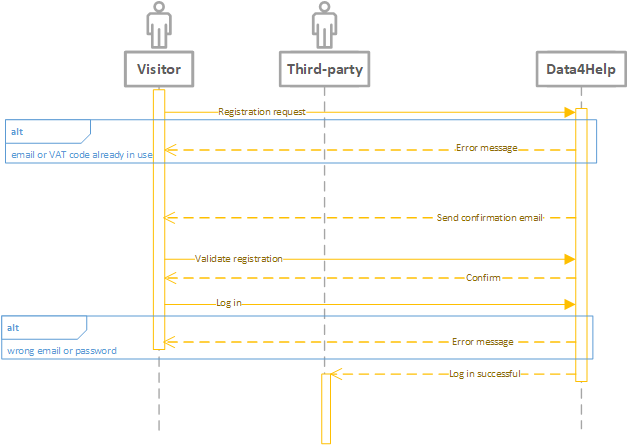
\includegraphics[scale=0.82]{pictures/RegistrationSequenceDiagram.png}}
                \caption{Sequence diagram representing the registration/log in phase of a Third-party}
                \label{fig:seq-diagram2}
            \end{figure}
            
            
        \subsubsection{Single user data request and subscription}
        %gian    
            
            
        \subsubsection{Single User data unsubscription}
            After a successful subscription request, both Third-party or Individual can make a request in order to break the subscription to the specified data.

            \begin{table}[H]
            	\centering
                
                \begin{tabular}{|p{3cm}|p{8.2cm}|}
                    \hline
                    \textbf{Actors} &  \begin{itemize}
                                            \item Third-party
                                            \item Individual
                                        \end{itemize}\\
                     \hline
                    \textbf{Goals} & \\ 
                     \hline
                    \textbf{Entry Condition} & Third-party is logged in and has previously subscribed to the Individual's data.\\
                     \hline
                    \textbf{Events Flow} & \begin{enumerate}
                                                \item The Third-Party or Individual access to the subscription page and select the subscription to be cancelled.
                                                \item The Third-party or the Individual presses ``\emph{Unsubscribe}" button.
                                                \item The system deletes the Third-party subscription and sends an email to both Third-party and Individual.
                                            \end{enumerate}\\
                     \hline
                    \textbf{Exit Condition} & The Third-party is not subscribed anymore, but it has access to the previously received data. \\
                     \hline
                    \textbf{Exception} & There are no exceptions. \\
                     \hline
                \end{tabular}  
            \end{table} 
            
        \subsubsection{Aggregated user data request and subscription}
            Third-parties can perform group queries, asking for data coming from several Individuals that are within certain parameters specified by them (geographical areas, age, genre, time of the day). These requests are evaluated directly by D4H, that sends back the requested data only if the number of Individuals involved in the research is greater than 1000. If this is not the case, D4H sends an error message to the Third-party.

            \begin{table}[H]
            	\centering
                \begin{tabular}{|p{3cm}|p{8.2cm}|}
                    \hline
                    \textbf{Actors} &  \begin{itemize}
                        \item Third-party
                    \end{itemize} \\
                     \hline
                    \textbf{Goals} & \\ 
                     \hline
                    \textbf{Entry Condition} & The Third-party is logged in. \\
                     \hline
                    \textbf{Events Flow} & \begin{enumerate}
                        \item The Third-party clicks on the ``\emph{Aggregated data research}" button.
                        \item The Third-party inserts the parameters of interest.
                        \item The Third-party decides whether it wants to subscribe to this particular research by checking the specific box or not, then clicks on the ``\emph{Search}" button to have D4H perform the query.
                        \item \emph{Data4Help} does the research and evaluates the results.
                        \item D4H sends back the result to the Third-party.
                    \end{enumerate} \\
                     \hline
                    \textbf{Exit Condition} & The Third-party receives the requested information. \\
                     \hline
                    \textbf{Exception} & The number of Individuals involved in the query is lower                        than 1000, therefore D4H sends an error message back to the                      Third-party. \\
                     \hline
                \end{tabular}  
            \end{table}
            
        \subsubsection{Aggregated user data unsubscription}
        After a successful subscription to a group search, a Third-party can cancel it at any time if it does not wish to receive any further update. He will, however, still have access to the data collected until that point.
        
            \begin{table}[H]
            	\centering
                \begin{tabular}{|p{3cm}|p{8.2cm}|}
                    \hline
                    \textbf{Actors} &  \begin{itemize}
                        \item Third-party
                    \end{itemize} \\
                     \hline
                    \textbf{Goals} & \\ 
                     \hline
                    \textbf{Entry Condition} & The Third-party is logged in and has previously subscribed to a group search. \\
                     \hline
                    \textbf{Events Flow} & \begin{enumerate}
                        \item The Third-Party accesses to the subscription page and selects the subscription to be cancelled.
                        \item The Third-party presses the ``\emph{Unsubscribe}" button.
                        \item The system deletes the Third-party subscription and sends an email to it for confirmation.
                    \end{enumerate} \\
                     \hline
                    \textbf{Exit Condition} & The Third-party is not subscribed anymore, but it has access to the previously received data. \\
                     \hline
                    \textbf{Exception} & There are no exceptions. \\
                     \hline
                \end{tabular}  
            \end{table}        
        
        
        \subsubsection{Data Collection}
            
            Upon registration, Individuals allows the D4H system to collect their data and store them. To gather data, it's mandatory to have a device (smart-watch or fitness-band). 
            
            \begin{table}[H]
            	\centering
                
                \begin{tabular}{|p{3cm}|p{8.2cm}|}
                    \hline
                    \textbf{Actors} & \begin{itemize}
                        \item Individual
                    \end{itemize} \\
                     \hline
                    \textbf{Goals} & \\ 
                     \hline
                    \textbf{Entry Condition} & The user is correctly registered and logged into the D4H system.\\
                     \hline
                    \textbf{Events Flow} & \begin{enumerate}
                                                \item Smart-watches or fitness-band samples specific data.
                                                \item This device sends acquired data to D4H system.
                                                \item The system stores data and makes them visible to the owner Individual.
                                            \end{enumerate}\\
                     \hline
                    \textbf{Exit Condition} & The individual has personal data storage in his D4H account.\\
                     \hline
                    \textbf{Exception} & If the associate device (smart-watch or fitness-bend) doesn't work or does not send data anymore an exception will be handled by the system ... come?\\
                     \hline
                \end{tabular}  
            \end{table} 
            
    \subsection{Automated SOS}
            
        \subsubsection{Subscription Request}
            
            Every Individual, user registered to D4H, can ask for subscription to Automated SOS service, but only Elderly people will be allowed to use it.
            
            \begin{table}[H]
            	\centering
                
                \begin{tabular}{|p{3cm}|p{8.2cm}|}
                    \hline
                    \textbf{Actors} & \begin{itemize}
                        \item Individual
                    \end{itemize} \\
                     \hline
                    \textbf{Goals} & \\ 
                     \hline
                    \textbf{Entry Condition} & The user has a D4H account. \\
                     \hline
                    \textbf{Events Flow} & \begin{enumerate}
                                               \item The user logs into his D4H personal account.
                                               \item The Individual presses on
                                               ``\emph{AutomatedSOS service}", in order to make a new subscription request.
                                               \item The ASOS System checks if the petitioner is at least 65 years old.
                                               \item If verified, the user is now subscribed.
                                           \end{enumerate}\\
                     \hline
                    \textbf{Exit Condition} & The Individual is now subscribed to Automated SOS service.\\
                     \hline
                    \textbf{Exception} & If the petitioner is less then 65 years old, the system handle the exception, sending him an error message. \\
                     \hline
                \end{tabular}  
            \end{table} 
            
            
    \subsection{Track4Run}
            
        \subsubsection{Run organisation}
            
            The T4R system allows registered organisers to organise a run. They have to specify the time and the place, but it is not possible to add if there is another, already stored, race in the same place and at the same time. Different runs at the same time but different place are allowed.
            
            \begin{table}[H]
            	\centering
                
                \begin{tabular}{|p{3cm}|p{8.2cm}|}
                    \hline
                    \textbf{Actors} & \begin{itemize}
                        \item Organiser
                    \end{itemize} \\
                     \hline
                    \textbf{Goals} & \\ 
                     \hline
                    \textbf{Entry Condition} & Organiser must have an organiser account in T4R system.\\
                     \hline
                    \textbf{Events Flow} & \begin{enumerate}
                                                \item The organiser logs into his/her personal account.
                                                \item He presses on ``\emph{New Run}" button.
                                                \item The organiser specifies date, time, place and the maximum number of participants.
                                                \item The system creates this new run, stores it and sends a notification email to the organiser.
                                            \end{enumerate}\\
                     \hline
                    \textbf{Exit Condition} & A new race has been created.\\
                     \hline
                    \textbf{Exception} & If there is another stored race with the same data, time and place, the system handles the exception, showing an error message to the organiser. \\
                     \hline
                \end{tabular}  
            \end{table} 
            
            
        \subsubsection{Participant tracking}
            
            Every Visitor, registered or not, is able to track participants on a map during the race and, if there is more then one run at the same time, they can choose which run to watch. To provide this service, the system interacts with Google Maps.
            
            \begin{table}[H]
            	\centering
                
                \begin{tabular}{|p{3cm}|p{8.2cm}|}
                    \hline
                    \textbf{Actors} & \begin{itemize}
                                            \item Visitor
                                            \item Map service
                                        \end{itemize}\\
                     \hline
                    \textbf{Goals} & \\ 
                     \hline
                    \textbf{Entry Condition} & There is no entry condition \\
                     \hline
                    \textbf{Events Flow} & \begin{enumerate}
                                                \item The visitor launches the application.
                                                \item They press on the ``\emph{Track runners}" button.
                                                \item The system shows the list of current runs.
                                                \item The visitor selects the run of interest.
                                                \item The system asks for map and runners positions to the map service.
                                                \item The map service sends to the system map and runners location.
                                                \item The system shows the map with all runners current position.
                                            \end{enumerate}\\
                     \hline
                    \textbf{Exit Condition} & Visitors are now able to see runners on a map.\\
                     \hline
                    \textbf{Exception} & If there are no runs in that moment, the system handles the exception, showing a notification message.\\
                     \hline
                \end{tabular}  
            \end{table} 
        